\chapter{Introduzione}

\section{Contesto e Motivazioni}

Tutti gli esseri viventi sono costituiti da cellule, piccole fabbriche biochimiche
che attraverso dei metabolismi consumano energia per esistere.

Studiare le cellule e il loro funzionamento è fondamentale per comprendere malattie nel corpo umano, come il cancro.

Una cellula nella sua interezza è un sistema biologico governato da reti complesse di interazioni tra molecole come proteine, metaboliti e acidi nucleici.

Tuttavia si possono studiare solo piccoli parti di questi network metabolici, ovvero i pathway che vanno a studiare una specifica funzione di una cellula. 

Un modello biologico è formato da molecole e reazioni come mostrato in figura \ref{fig:paziente_virtuale}. 

Esistono online database di pathway che possono essere resi simulabili modellando le reazioni come equazioni differenziali ordinarie (ODE).

Per questo tirocinio è stato utilizzato reactome \cite{milacic2024reactome}.

L'accuratezza di queste simulazioni dipende in modo cruciale dalle costanti cinetiche che governano le reazioni. Tali parametri risultano spesso difficili o impossibili da misurare sperimentalmente, lasciando un ampio margine di incertezza nei modelli.

Però esiste il concetto di \textbf{paziente virtuale} inteso come una collezione di
modelli computazionali che rappresentano diversi possibili scenari biologici compatibili con le conoscenze disponibili.

\begin{figure}[htbp]
    \centering
    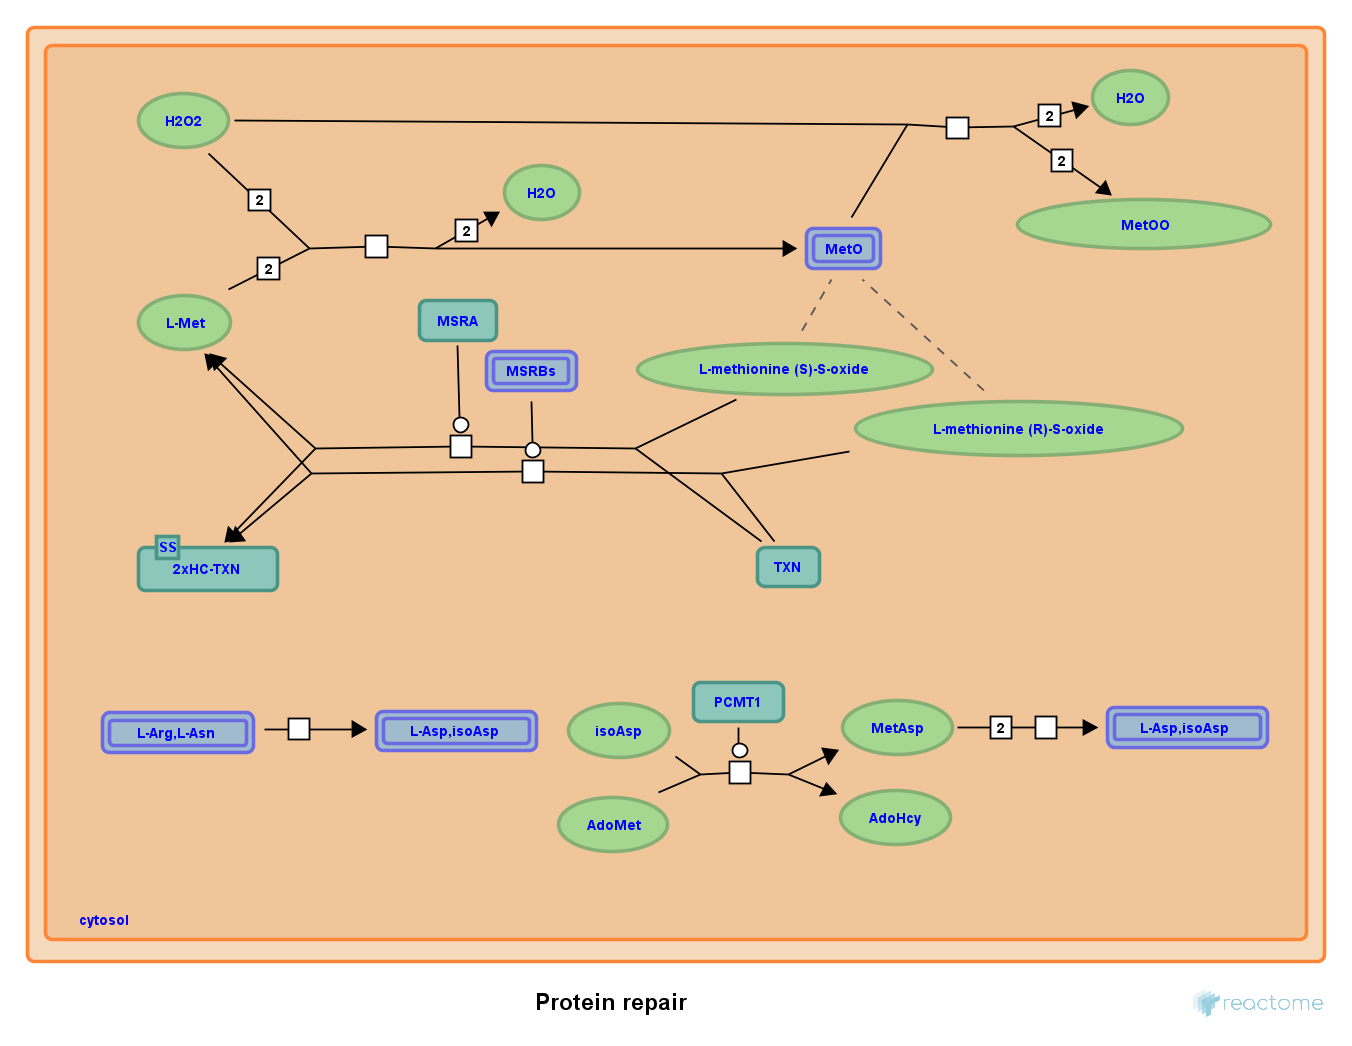
\includegraphics[width=0.8\textwidth]{R-HSA-5676934.png}
    \caption{Rappresentazione schematica di un modello bioligico. Le freccie sono le reazioni che collegano i reattanti con i prodotti delle reazioni.}
    \label{fig:paziente_virtuale}
\end{figure}

\section{Contributi}

Con questa relazione di tirocinio, si vuole presentare un software che, dato un modello biologico, permette di individuare pazienti virtuali plausibili, ovvero insiemi di parametri coerenti con i vincoli biologici.

In particolare, il lavoro introduce un framework computazionale per l'esplorazione degli spazi di parametri cinetici in reti biochimiche. I contributi principali sono:

\begin{enumerate}
    \item Algoritmo per verificare l'esistenza di assegnazioni dei parametri che soddisfino le condizioni di stato stazionario e riproducano l'ordinamento relativo delle concentrazioni delle specie.
    \item Implementazione software integrata con librerie di simulazione consolidate, che garantisca riproducibilità ed estendibilità.
    \item Implementazione di un algoritmo evolutivo di OpenAI per l'ottimizzazione black-box.
\end{enumerate}

\section{Stato dell'arte}

% TODO: mettere riferimento ad equazioni differenziali

L'approccio di usare equazioni differenziali per modellare sistemi biochimici è una pratica molto diffusa nella letteratura. La dinamica delle reti biochimiche viene descritta tramite equazioni differenziali ordinarie, che permettono di rispettare i vincoli quantitativi e temporali delle reazioni chimiche.

Invece un approccio alternativo alla simulazione dei sistemi biologici con equazioni differenziali è quello basato sui network booleani \cite{boolean_network1} \cite{boolean_network2} \cite{boolean_network3}. In questo caso, le reazioni biochimiche sono fortemente semplificate: ogni proteina può essere soltanto attiva o inattiva e le interazioni sono ridotte a regole logiche. Spesso si assume che tutte le reazioni avvengano alla stessa velocità e che i nodi della rete possano cambiare stato in maniera sincrona. In alcuni modelli, si ipotizza persino che durante la simulazione la velocità relativa delle reazioni possa variare, ma questa assunzione non è coerente con i vincoli fisici: se una reazione è intrinsecamente veloce, lo rimane, e non può diventare lenta.

\section{Struttura della Relazione di Tirocinio}

\begin{itemize} % TODO: aggiungi riferimenti
    \item Capitolo 2 presenta il background teorico sulla modellazione di reti biochimiche.
    \item Capitolo 3 descrive la formulazione del problema e i vincoli usati per definire le assegnazioni di parametri ammissibili.
    \item Capitolo 4 Illustra l'algoritmo di OpenAI come uno dei possibili per trovare i parametri
    \item Capitolo 5 Introduce la progettazione del software e le dipendenze utilizzate per crearlo.
    \item Capitolo 6 si presentano degli utilizzi su 5 modelli biologici presi da Reactome.
    \item Capitolo 7 considerazioni finali e possibili sviluppi futuri.
\end{itemize}